% Options for packages loaded elsewhere
\PassOptionsToPackage{unicode}{hyperref}
\PassOptionsToPackage{hyphens}{url}
%
\documentclass[
]{article}
\usepackage{amsmath,amssymb}
\usepackage{iftex}
\ifPDFTeX
  \usepackage[T1]{fontenc}
  \usepackage[utf8]{inputenc}
  \usepackage{textcomp} % provide euro and other symbols
\else % if luatex or xetex
  \usepackage{unicode-math} % this also loads fontspec
  \defaultfontfeatures{Scale=MatchLowercase}
  \defaultfontfeatures[\rmfamily]{Ligatures=TeX,Scale=1}
\fi
\usepackage{lmodern}
\ifPDFTeX\else
  % xetex/luatex font selection
  \setmainfont[]{Times New Roman}
\fi
% Use upquote if available, for straight quotes in verbatim environments
\IfFileExists{upquote.sty}{\usepackage{upquote}}{}
\IfFileExists{microtype.sty}{% use microtype if available
  \usepackage[]{microtype}
  \UseMicrotypeSet[protrusion]{basicmath} % disable protrusion for tt fonts
}{}
\makeatletter
\@ifundefined{KOMAClassName}{% if non-KOMA class
  \IfFileExists{parskip.sty}{%
    \usepackage{parskip}
  }{% else
    \setlength{\parindent}{0pt}
    \setlength{\parskip}{6pt plus 2pt minus 1pt}}
}{% if KOMA class
  \KOMAoptions{parskip=half}}
\makeatother
\usepackage{xcolor}
\usepackage[margin=1in]{geometry}
\usepackage{graphicx}
\makeatletter
\def\maxwidth{\ifdim\Gin@nat@width>\linewidth\linewidth\else\Gin@nat@width\fi}
\def\maxheight{\ifdim\Gin@nat@height>\textheight\textheight\else\Gin@nat@height\fi}
\makeatother
% Scale images if necessary, so that they will not overflow the page
% margins by default, and it is still possible to overwrite the defaults
% using explicit options in \includegraphics[width, height, ...]{}
\setkeys{Gin}{width=\maxwidth,height=\maxheight,keepaspectratio}
% Set default figure placement to htbp
\makeatletter
\def\fps@figure{htbp}
\makeatother
\setlength{\emergencystretch}{3em} % prevent overfull lines
\providecommand{\tightlist}{%
  \setlength{\itemsep}{0pt}\setlength{\parskip}{0pt}}
\setcounter{secnumdepth}{-\maxdimen} % remove section numbering
\usepackage{booktabs}
\usepackage{longtable}
\usepackage{array}
\usepackage{multirow}
\usepackage{wrapfig}
\usepackage{float}
\usepackage{colortbl}
\usepackage{pdflscape}
\usepackage{tabu}
\usepackage{threeparttable}
\usepackage{threeparttablex}
\usepackage[normalem]{ulem}
\usepackage{makecell}
\usepackage{xcolor}
\ifLuaTeX
  \usepackage{selnolig}  % disable illegal ligatures
\fi
\IfFileExists{bookmark.sty}{\usepackage{bookmark}}{\usepackage{hyperref}}
\IfFileExists{xurl.sty}{\usepackage{xurl}}{} % add URL line breaks if available
\urlstyle{same}
\hypersetup{
  pdftitle={HW1-OLS\_Regression},
  hidelinks,
  pdfcreator={LaTeX via pandoc}}

\title{HW1-OLS\_Regression}
\author{}
\date{\vspace{-2.5em}2023-10-19}

\begin{document}
\maketitle

\hypertarget{introduction}{%
\section{Introduction}\label{introduction}}

Complex real estate markets influence the prices of homes, and
determining what features are most impactful to the value goes beyond
physical characteristics. In this analysis, we use ordinary least
squares regression to investigate the variation in median home sales
prices for Census block groups in the city of Philadelphia, PA. We use a
multivariate linear regression model to determine the correlation
between median home value for owner occupied housing units in block
groups and four predictive variables:

\begin{itemize}
\tightlist
\item
  proportion of residents in a block group with at least a bachelor's
  degree;
\item
  proportion of housing units that are vacant;
\item
  percent of housing units that are detached single family houses; and
\item
  number of households living in poverty
\end{itemize}

We include the proportion of residents in a block group with at least a
bachelor's degree because previous research has indicated that there is
a correlation between income and educational attainment\footnote{Sean
  Reardon, The Widening Academic Achievement Gap Between the Rich and
  the Poor: New Evidence and Possible Explanations, Stanford University,
  \url{https://cepa.stanford.edu/sites/default/files/reardon\%20whither\%20opportunity\%20-\%20chapter\%205.pdf}}.
This correlation results in households that lack a higher education
degree having less wealth and are thus likely to only be able to
purchase homes in areas with lower median home values.

The proportion of housing units that are detached single family homes is
included as a predictor, because detached single family homes tend to be
larger and there is typically a correlation between home size and
property value.

We include the percentage of lots which are vacant as a predictor
because previous research indicates that there is a correlation between
vacant lots and median home sales prices in Philadelphia. Gravin er all
note that there are 40,000 vacant parcels in Philadelphia and most of
these are concentrated in low income areas\footnote{Eugenia Garvin et.
  all, More Than Just An Eyesore: Local Insights And Solutions on Vacant
  Land And Urban Health, Journal of Urban
  Health,\url{https://link.springer.com/article/10.1007/s11524-012-9782-7}}.

We include the number of households with income below 100\% poverty
levels because low income households are less likely to be able to
afford homes in expensive areas.

\hypertarget{methods}{%
\section{Methods}\label{methods}}

\hypertarget{data-cleaning}{%
\subsection{Data Cleaning}\label{data-cleaning}}

The data set used in our analysis contains information from the 2000 US
Census for Philadelphia, with neighborhood characteristic variables
included for 1,720 block groups. Our analysis incorporates the following
variables:

\begin{itemize}
\tightlist
\item
  POLY\_ID: Census Block Group ID
\item
  MEDHVAL: Median value of all owner occupied housing units
\item
  PCBACHMORE: Proportion of residents in a block group with at least a
  bachelor's degree
\item
  PCTVACANT: Proportion of housing units that are vacant
\item
  PCTSINGLES: Percent of housing units that are detached single family
  houses
\item
  NBELPOV100: Number of households with incomes below 100\% poverty
  level (i.e., number of households living in poverty)
\item
  MEDHHINC: Median household income
\end{itemize}

The original data set included 1,816 block groups and was cleaned based
on the following criteria, which reduced to the total number of
observations to 1,720:

\begin{itemize}
\tightlist
\item
  Block groups where population is less than 40 people
\item
  Block groups without housing units
\item
  Block groups where the median house value is lower than \$10,000
\item
  One North Philadelphia block group which had a very high median house
  value (over \$800,000) and a very low median household income (less
  than \$8,000)
\end{itemize}

\hypertarget{exploratory-data-analysis}{%
\subsection{Exploratory Data Analysis}\label{exploratory-data-analysis}}

We will examine the summary statistics and distributions of the data
set's variables, including the mean and standard deviation of our
dependent variable and predictor variables.

As part of our exploratory data analysis, we will examine the Pearson
correlations between the predictors. A Pearson correlation, denoted in
this analysis by ``r'', is a standardized measurement of the strength
and direction of the linear relationship between two variables. The
correlation between two variables is calculated using the following
equation:

\[r=\frac{1}{n-1}\sum_{i=1}^{n}\left(\frac{x_i-x ̅}{s_x}\right)\left(\frac{y_i-y ̅}{s_x}\right)\]

A Pearson correlation value ranges between -1 to 1, with no units of
measurement attached, and the observed variables are interchangeable
between the x axis and y axis. A value of -1 represents a perfect
negative linear relationship and a value of 1 represents a perfect
positive linear relationship - in either case, points on a graph would
appear in a straight line with either a negative or positive slope,
respectively. A value of 0 indicates that there is no linear
relationship between two variables. However, a different type of
relationship can exist, such as an exponential or quadratic
relationship, that the Pearson correlation does not measure - in those
cases, a Spearman correlation would be more appropriate to calculate.

\hypertarget{multiple-regression-analysis}{%
\subsection{Multiple Regression
Analysis}\label{multiple-regression-analysis}}

Ordinary least square (OLS) regression is a statistical method used to
examine the linear relationship between a variable of interest
(dependent variable) and one or more explanatory variables (predictors).
This type of regression tests the strength of the relationship, the
direction of the relationship (positive, negative, or no relationship)
and goodness of model fit - how well a model will predict a future set
of observations. Regressions can also calculate the amount that the
dependent variable changes when a predictor variable changes by one unit
(holding all other predictors constant). However, if an explanatory
variable is a significant predictor of the dependent variable, it does
not imply causation.

When more than one predictor is present, multiple regression is used. In
a multiple regression analysis, there are \(K>1\) predictors, so rather
than getting a line in 2 dimensions from a simple linear regression,
there is instead a surface in \(K+1\) dimensions (\(+1\) accounts for
the dependent variable). Here, each independent variable will have its
own slope coefficient which indicates the relationship of that
particular predictor with the dependent variable, controlling for all
other independent variables in the regression.

To examine the relationship between median house values and several
neighborhood characteristics, we run a multiple regression. Using
Philadelphia data at the Census block group level, we regressed the
natural log of the median value of all owner occupied housing units
(LNMEDHVAL) on the following variables for each block group:

\begin{itemize}
\tightlist
\item
  The proportion of housing units that are vacant (PCTVACANT)
\item
  The percent of housing units that are detached single family homes
  (PCTSINGLES),
\item
  The proportion of residents in a block group with at least a
  bachelor's degree (PCTBACHMOR), and
\item
  The natural log of the number of households with incomes below 100\%
  poverty level (LNMEDHVAL).
\end{itemize}

The equation is stated as:

\begin{multline*}

$$LNMEDHHINC=\\β_0+β_1 PCTVACANT+β_2 PCTSINGLES+β_3 PCTBACHMOR+β_4 LNNBELPOV100+ ε $$
\end{multline*}

Performing a logarithmic transformation on the dependent variable
MEDHVAL and one the independent variables NBELPOV100 helps us to achieve
better normality of residuals, which is a core assumption when running
an OLS regression that we discuss in greater detail in the regressions
assumptions section of the study. The Beta coefficient β\_i of each
predictor is interpreted as the amount by which the dependent variable
changes as the independent variable increases by one unit, holding all
other variables constant. The sign indicates whether the relationship
between the dependent variable and the independent variables is positive
(direct) or negative (inverse). It is important to look at the sign and
value of β\_i when the coefficient is statistically significant and
different from zero. The β\_i is considered statistically significant
and different from zero when the p-value falls below our alpha threshold
of 0.05. The variable ε is commonly referred to as the residual term or
random error term in the model. The residual term ε allows the
regression line to fall above (ε \textgreater{} 0) or below (ε
\textless{} 0) the actual data points. ε is the difference between
observed values of y and the values of y predicted by the regression
model (denoted by y ̂).

\hypertarget{regression-assumptions}{%
\subsubsection{Regression Assumptions}\label{regression-assumptions}}

Prior to making conclusions about the model estimates or using the model
for predictions, certain assumptions must be met. These assumptions
include linearity, independence of observations, normality of residuals,
homoscedasticity, and no multicollinearity.

\textbf{Linearity} assumes that there is a linear relationship between
the dependent variable \(y\) and each of the predictors \(x\). Linearity
can be checked by creating scatterplots between y and each of the
predictors.

\textbf{Independence of observations} assumes that there should be no
spatial, temporal, or other forms of dependence in the data. This means
that each observation in the data must be independent of the others. In
order to test for independence of observations, one can examine the
Moran's I value for the residuals or the values of \(y\) to examine
whether regression residuals, or the dependent variable itself, are
spatially autocorrelated.

\textbf{Normality of residuals} is violated when either the dependent
variable or independent variables themselves are distributed
non-normally, or the linearity assumption is violated. This assumption
is not as essential to follow as the three previously stated
assumptions, especially when analyzing a data set with a large sample
size. In this context, a large sample size is generally defined as
having 30+ observations with 10 additional observations for every
additional predictor after the first one. One can test for this
assumption by looking at the histogram of residuals to see if they are
normal.

\textbf{No homoscedasticity} refers to the variance of the residuals ε
being constant regardless of the values of each \(x\) (or the values of
\(\widehat{y}\), i.e., values of y predicted by the model).
Heteroscedasticity is present when this assumption is violated, which
occurs when the residuals ε differ across all values of the independent
variables and means that there is systematic under-or over-predictions
happening in the model. This assumption can be checked by looking at
scatterplots of standardized residuals against each predictor to see if
variance of residuals remains the same for different values of each
predictor.

\textbf{No multicollinearity} only applies to multiple regression - no
multicollinearity occurs when predictor variables are not strongly
correlated with each other. Multicollinearity is when two or more
predictors are very strongly correlated with each other: \(r > 0.8\) or
\(r < -0.8\). If multicollinearity is present in a model, it will become
difficult for the model to estimate the relationship between each
predictor and the dependent variable independently, making it difficult
to identify significant predictors. One can check for this assumption by
reviewing a correlation matrix of the predictors to check if \(r > 0.8\)
or \(r < -0.8\) for two predictors. If two or more predictors are
strongly correlated, only one of these correlated predictors should be
included in the regression model.

\hypertarget{multiple-regression-parameters-estimation}{%
\subsubsection{Multiple Regression Parameters \&
Estimation}\label{multiple-regression-parameters-estimation}}

Performing multiple regression requires one to estimate the values for a
critical set of parameters. These parameters include \(σ^2\), which
determines the amount of variability inherent in a regression model; a
regression constant \(β_0\); and one regression coefficient \(β_i\) for
each independent variable in the model. The regression constant (i.e.,
the intercept) \(β_0\) represents the mean value of the dependent
variable when all independent variables are equal to 0. The regression
coefficient, as stated previously, is interpreted as the amount by which
the dependent variable changes as the independent variable increases by
one unit, holding all other variables constant. In multiple regression
we estimate these parameters by finding the values \(β_0\) and \(β_i\)
that minimize the Sum of Squared Errors (SSE) of prediction, the amount
of variability in y that is not explained when accounting for the
predictors in the model. SSE will produce the Least Square estimates
\(\widehat{\beta_0}\) \& \(\widehat{\beta_k}\). The equation for SSE is
stated as:

\[SSE = \sum(y_i - \hat{y_i})^2 = \sum[y_i - (\hat\beta_0 + \hat\beta_1x_{1i} + \hat\beta_2x_{2i} + ... + \hat\beta_kx_{ki})]^2 \]

For multiple regression, the equation for \(σ^2\) is stated as
\(σ^2 = \frac{SSE}{n-(k+1)} = MSE\), where k = \# predictors and n = \#
observations. Here, MSE stands for mean squared error.

\hypertarget{coefficient-of-multiple-determination-r2}{%
\subsubsection{\texorpdfstring{Coefficient of Multiple Determination
\(R^2\)}{Coefficient of Multiple Determination R\^{}2}}\label{coefficient-of-multiple-determination-r2}}

\(R^2\) is the proportion of observed variance in the dependent variable
y that is explained by the model by all k predictors - it is often
referred to as the coefficient of multiple determination. Higher values
of R2 are indicative of a better model. \(R^2\) is calculated as
\(R^2 = 1 - \frac{SSE}{SST}\), where SSE is the sum of squared residuals
and SST is the total variability in the dependent variable. Adjusted
\(R^2\) is the \(R^2\) value adjusted for the number of predictors in
the model and is used to account for a high number of predictor
variables in the model, which can increase \(R^2\) based on presence
alone. Larger values for Adjusted \(R^2\), like \(R^2\), are also
indicative of a better model. The equation for Adjusted \(R^2\) is
stated as:

\[R_{adj}^2 = \frac{(n-1)R^2 - k}{n-(k+1)}\]

\hypertarget{hypothesis-testing}{%
\subsubsection{Hypothesis Testing}\label{hypothesis-testing}}

For hypothesis testing, we examine a baseline - the null hypothesis -
compared to an alternative hypothesis. To examine the overall
significance of our regression model, we first use the F-Ratio to test
the null hypothesis \(H_0: β_i=0\) that none of the independent
variables in the model are a significant predictor of the dependent
variable (LNMEDHVAL) against the alternative hypothesis \(H_a: β_i≠0\)
that at least one of the independent variables is a significant
predictor of the dependent variable (LNMEDHVAL). Second, we use T-test
hypothesis testing to determine the significance of each chosen
predictor on our dependent variable LNMEDHVAL - \(β_1PCTVACANT\),
\(β_2PCTSINGLES\), \(β_3PCTBACHMOR\), and \(β_4LNNBELPOV100\).

PCTVACANT:

\begin{itemize}
\tightlist
\item
  \(H_0: β_i=0\): Implies that the variable PCTVACANT is not a
  significant predictor of the dependent variable (LNMEDHVAL).
\item
  \(H_a: β_i≠0\): Implies that the variable PCTVACANT is a significant
  predictor of the dependent variable (LNMEDHVAL) for
  \(1 \leq i \leq k\)
\end{itemize}

PCTSINGLES:

\begin{itemize}
\tightlist
\item
  \(H_0: β_i=0\): Implies that the variable PCTSINGLES is not a
  significant predictor of the dependent variable (LNMEDHVAL).
\item
  \(H_a: β_i≠0\): Implies that the variable PCTSINGLES is a significant
  predictor of the dependent variable (LNMEDHVAL).
\end{itemize}

PCTBACHMOR:

\begin{itemize}
\tightlist
\item
  \(H_0: β_i=0\): Implies that the variable PCTBACHMOR is not a
  significant predictor of the dependent variable (LNMEDHVAL).
\item
  \(H_a: β_i≠0\): Implies that the variable PCTBACHMOR is a significant
  predictor of the dependent variable (LNMEDHVAL).
\end{itemize}

LNNBELPOV100: - \(H_0: β_i=0\): Implies that the variable LNNBELPOV100
is not a significant predictor of the dependent variable (LNMEDHVAL). -
\(H_a: β_i≠0\): Implies that the variable LNNBELPOV100 is a significant
predictor of the dependent variable (LNMEDHVAL).

\hypertarget{additional-analyses}{%
\subsection{Additional Analyses}\label{additional-analyses}}

\hypertarget{stepwise-regression}{%
\subsubsection{Stepwise Regression}\label{stepwise-regression}}

Stepwise regression is a data mining method which selects predictors
based on the following criteria:

\begin{itemize}
\tightlist
\item
  P-values are below a certain threshold (variables where the P-value
  \textless{} 0.1)
\item
  The smallest value of the Akaike Information Criterion (AIC), which
  measures the relative quality of statistical models
\end{itemize}

There are a number of limitations when using Stepwise regression, which
include:

\begin{itemize}
\tightlist
\item
  The final model is not guaranteed to be optimal in any specified sense
\item
  The stepwise procedure produces a single final model, although there
  are often several equally good models
\item
  It does not consider a researcher's knowledge of the predictors
\item
  While the order in which the variables are removed or added can
  provide valuable information, it is important not to over-interpret
  the order
\item
  One should not conclude that all the important variables for
  predicting \(y\) have been identified or that all unimportant
  variables have been eliminated
\end{itemize}

\hypertarget{k-fold-cross-validation}{%
\subsubsection{K-Fold Cross-Validation}\label{k-fold-cross-validation}}

The k-Fold Cross-Validation approach involves randomly dividing the set
of observations into \(k\) groups (or folds) of approximately equal
size. In practice, typical folds to use are \(k=5\) or \(k=10\). The
first fold is treated as a validation set and the model is fitted on the
remaining \(k-1\) folds (training data set). The MSE is then computed on
the observations in the held-out fold. The procedure is repeated \(k\)
times with a different fold treated as the validation set. This process
results in \(k\) estimates of MSE.

The k-fold MSE estimate is computed by averaging the MSEs across the k
folds. The k-fold root mean squared error (RMSE) is computed as the
square root of the MSE:
\(RMSE = \sqrt{\frac{\sum_{i=1}^n \epsilon_i^2}{n}}\). RMSE values can
be compared across different models, with the model that has the
smallest RMSE considered the best model.

\hypertarget{software}{%
\subsection{Software}\label{software}}

This report used the open source software R to conduct statistical
analyses.

\hypertarget{results}{%
\section{Results}\label{results}}

\hypertarget{exploratory-results}{%
\subsection{Exploratory Results}\label{exploratory-results}}

\hypertarget{summary-statistics}{%
\subsubsection{Summary Statistics}\label{summary-statistics}}

The following table provides the mean and standard deviation for our
dependent variable (median house value) and our four independent
variables. The average median home value for census block groups in
Philadelphia is \$66,287.73 and the standard deviation is \$60,006 USD.
The standard deviation is nearly equal to the median, which indicates a
large amount of variability in average home sale prices across block
groups in the city.

\begin{table}
\centering
\begin{tabular}[t]{l|r|r}
\hline
Variable & Mean & Standard Deviation\\
\hline
Median Houme Value of all occupied housing units & 66287.733139 & 60006.075990\\
\hline
\% of Individuals with Bachelor Degrees or Higher & 16.081372 & 17.769558\\
\hline
\# Households Living in Poverty & 189.770930 & 164.318480\\
\hline
\% of Vacant Houses & 11.288529 & 9.628472\\
\hline
\% of Single House Units & 9.226473 & 13.249250\\
\hline
\end{tabular}
\end{table}

\hypertarget{quick-code-that-checks-which-variables-have-0-values-for-logarithmic-transformation}{%
\section{quick code that checks which variables have 0 values for
logarithmic
transformation}\label{quick-code-that-checks-which-variables-have-0-values-for-logarithmic-transformation}}

\hypertarget{histograms}{%
\subsubsection{Histograms}\label{histograms}}

\hypertarget{median-home-value-of-owner-occupied-housing-units}{%
\paragraph{Median Home Value of Owner-Occupied Housing
Units}\label{median-home-value-of-owner-occupied-housing-units}}

The two histograms below show the distribution of our dependent
variable, the median home values of owner occupied housing units by
block group before and after applying a natural log transformation. The
histogram without the natural log transformation peaks near \$75,000 and
is right-skewed - it does not have a normal distribution. After applying
a natural log transformation, the mean home value has a near normal
distribution with a peak around 11.

Our analysis will use a natural log transformation of median home sales
value as the independent variable because a core assumption of linear
regression is that variables are normally distributed. Using a normally
distributed variable can help mitigate issues resulting from a
non-linear relationship between our independent and dependent variables.
The natural log transformation is most widely used with positive-skewed
(i.e., right-skewed) data such as our dependent variable.


\includegraphics{HW1-Regression_files/figure-latex/hist_MEDHVAL-1.pdf}

\hypertarget{percent-of-population-with-a-bachelor-degree}{%
\paragraph{Percent of Population with a Bachelor
Degree:}\label{percent-of-population-with-a-bachelor-degree}}

The following histograms show the distribution of the percent of the
population with a bachelor's degree by block group before and after
applying a natural log transformation. The histogram without the natural
log transformation is right-skewed, and there are 143 block groups where
0\% of the population has a bachelor's degree.

After applying a natural log transformation, the 143 census blocks which
had a value of 0\% continue to have a value of 0. The distribution with
the natural log transformation applied is not normal, indicating that
the data has a zero-inflated distribution. Because both the variable
with and without the natural log transformation applied are both not
normal, we will use the variable without the natural log transformation
(PCTBACHMORE) for our model.

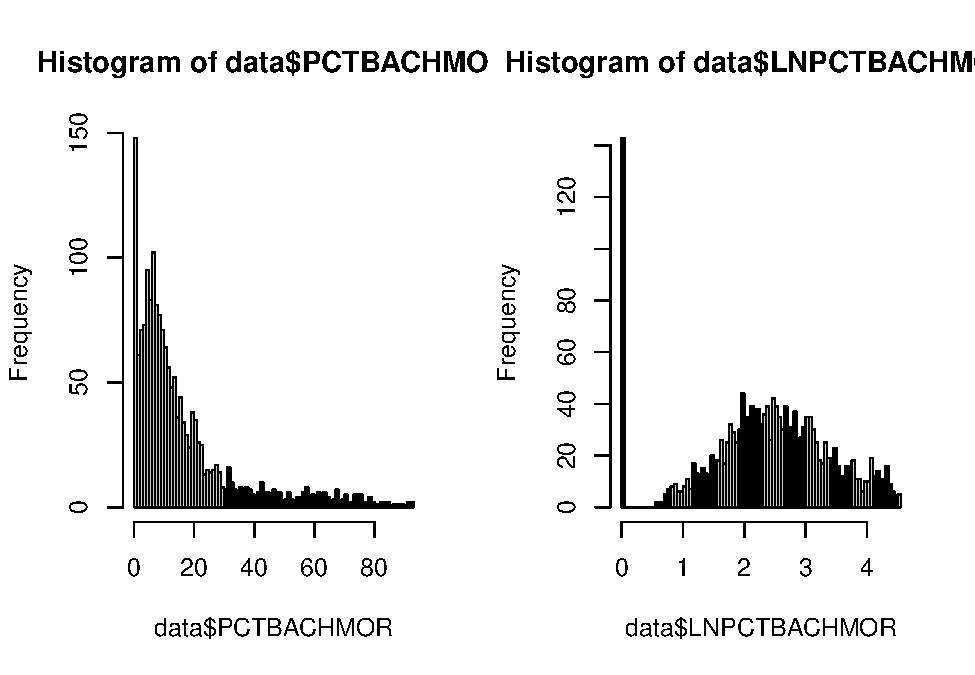
\includegraphics{HW1-Regression_files/figure-latex/hist_PCTBACHMOR-1.pdf}

\hypertarget{population-below-the-poverty-line}{%
\paragraph{Population Below the Poverty
Line}\label{population-below-the-poverty-line}}

The following histograms show the distribution of the population living
below the poverty line in each block group with and without a natural
log transformation applied. The histogram without the natural log
transformation is again right skewed and peaks around 100 households.
There is a very long tail to the right, and multiple outliers are
present. Notably, the maximum value is 1,267 households below the
poverty line in one census tract - which is more than six times larger
than the mean value.

After applying a natural log transformation, the variable displays a
distribution which is closer to a normal distribution. There is a clear
peak around 5.5, but the data is slightly skewed to the left and is
zero-inflated, but is closer to a normal distribution than the
distribution prior to transformation. Because the natural log
transformed variable is closer to a normal distribution we use the
natural log transformation of the Population Below the Poverty Line
(LNBELPOV100) in our regression. Additionally, the large positive skew
in the non natural log transformed data supports the usage of the
natural log transformed variable.

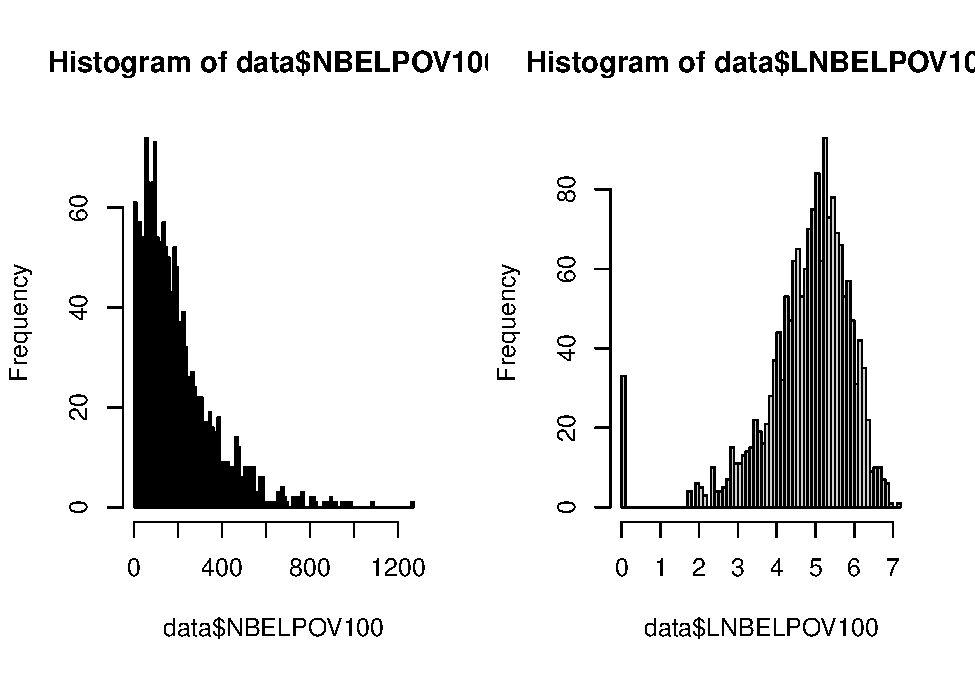
\includegraphics{HW1-Regression_files/figure-latex/hist_NBELPOV100-1.pdf}

\hypertarget{percent-of-vacant-housing-units}{%
\paragraph{Percent of Vacant Housing
Units}\label{percent-of-vacant-housing-units}}

The following histograms show the distribution for the percent of
housing units in a block group which are vacant with and without a
natural log transformation. The histogram without the natural log
transformation is right skewed and has a long tail, with multiple
outliers present. Additionally, there are 163 block groups where 0\% of
the housing units are vacant.

After applying the natural log transformation, the 163 block groups
which have a value of 0\% still have a value of 0. The presence of the
large number of block groups with a value of zero prevents the
distribution from being considered normal and results in a zero-inflated
distribution. Because neither distribution is normal, we use the
variable without the natural log transformation in our regression
analysis (PCTVACANT).

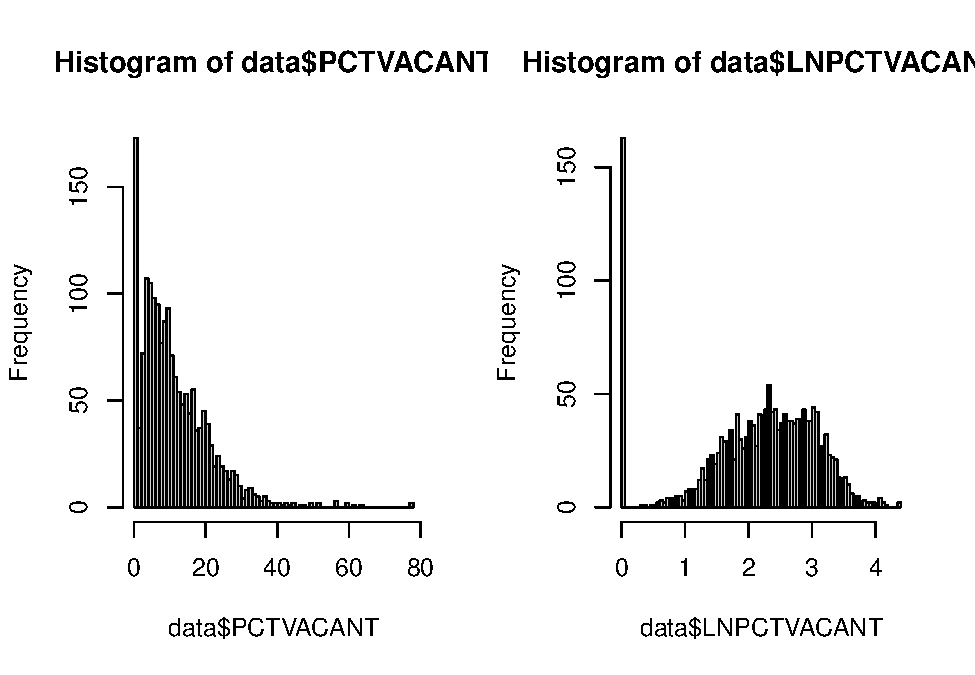
\includegraphics{HW1-Regression_files/figure-latex/hist_PCTVACANT-1.pdf}

\hypertarget{percent-of-detached-single-family-houses-units}{%
\paragraph{Percent of Detached Single Family Houses
Units}\label{percent-of-detached-single-family-houses-units}}

The following histograms show the distribution for the percent of
housing units that are detached single family homes by block group with
and without a natural log transformation. The histogram without the
natural log transformation is right-skewed, and the vast majority of
block groups (i.e: 1,548) have a percentage less than 20\% - 306 block
groups have a percentage of 0\%. There are 172 census block groups which
have percentages above 20\%, including three homes with values of 100\%.
The extreme outliers are likely a result of the inclusion of suburban
block groups in Northeast and Northwest Philadelphia, where most homes
are detached single family homes.

After applying a log transformation, the 306 block groups where the
percentage of detached single family homes is 0\% continue to have a
value of 0 resulting in a zero-inflated distribution. Because both the
natural log transformed and non-natural log transformed variable do not
have a normal distribution, we use the non-natural log transformed
variable in our regression analysis.

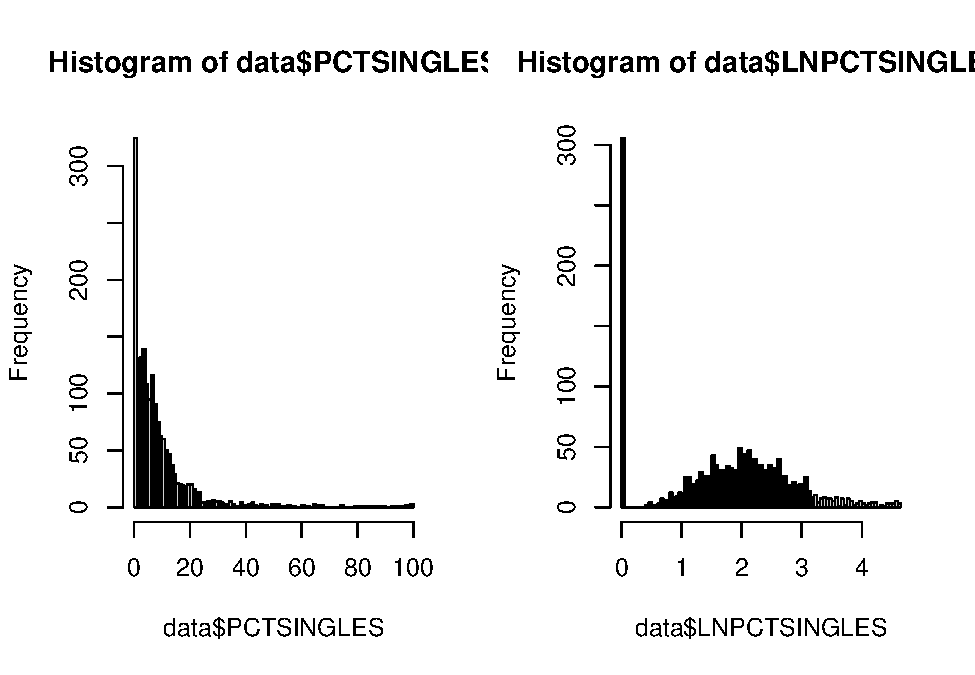
\includegraphics{HW1-Regression_files/figure-latex/hist_PCTSINGLES-1.pdf}

\hypertarget{maps}{%
\subsubsection{Maps}\label{maps}}

This section includes choropleth maps of our dependent and four
independent variables.

\hypertarget{map-of-dependent-variable}{%
\paragraph{Map of Dependent Variable}\label{map-of-dependent-variable}}

The following map shows our dependent variable, which is the median
house value of owner occupied units by block group with a natural log
transformation. We observe that the census tracts with the highest
median home values are primarily clustered in Center City and northwest
Philadelphia. The block groups with the lowest median home values are
located north of Center City and west of University City.

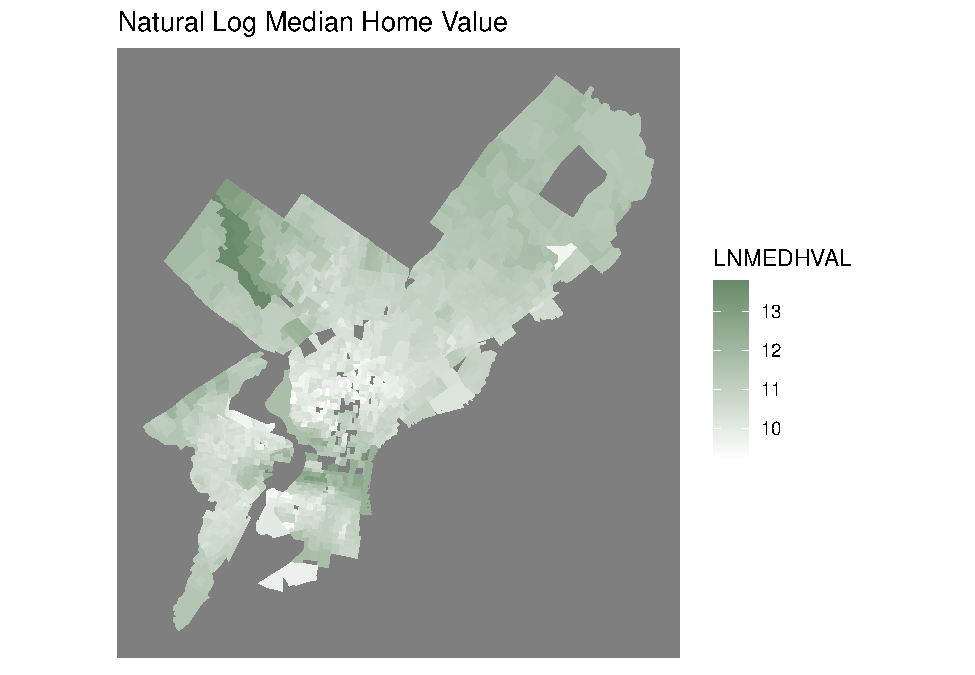
\includegraphics{HW1-Regression_files/figure-latex/LNMEDHVAL_map-1.pdf}

\hypertarget{maps-of-independent-variables}{%
\paragraph{Maps of Independent
Variables}\label{maps-of-independent-variables}}

The following maps show the spatial patterns on our four independent
variables: PCTBACHMOR, PCTVACANT, PCTSINGLES, and LNBELPOV100.

Based on a review of the maps, the PCTBACHMOR variable appears to be the
independent variable with the strongest correlation with our dependent
variable. Like our dependent variable, the percentage of residents with
a bachelor's degree is highest in Center City and northwest
Philadelphia. The areas with the lowest percentage of residents with a
bachelor degree are located west of University City and north of Center
City - these are the same areas where the natural log transformed median
home values are lowest.

Conversely, the PCTSINGLES variable appears to be less correlated with
our dependent variable. This is because the percent of housing units
that are detached single family homes tends to be low in Center City and
high in northwest Philadelphia, which are both neighborhoods with high
median home prices values.

The independent variables PCTBACHMOR and PCTVACANT appear to have strong
negative correlations, as areas with a high PCTVACANT rate also have a
low PCTBACHMOR rate. Conversely, areas with a high PCTBACHMOR rate have
a low PCTVACANT rate. This negative correlation indicates that there may
be multicollinearity between these two variables. We will check the
strength of this correlation using the Pearson correlation to determine
if this multicollinearity could be an issue in our regression.

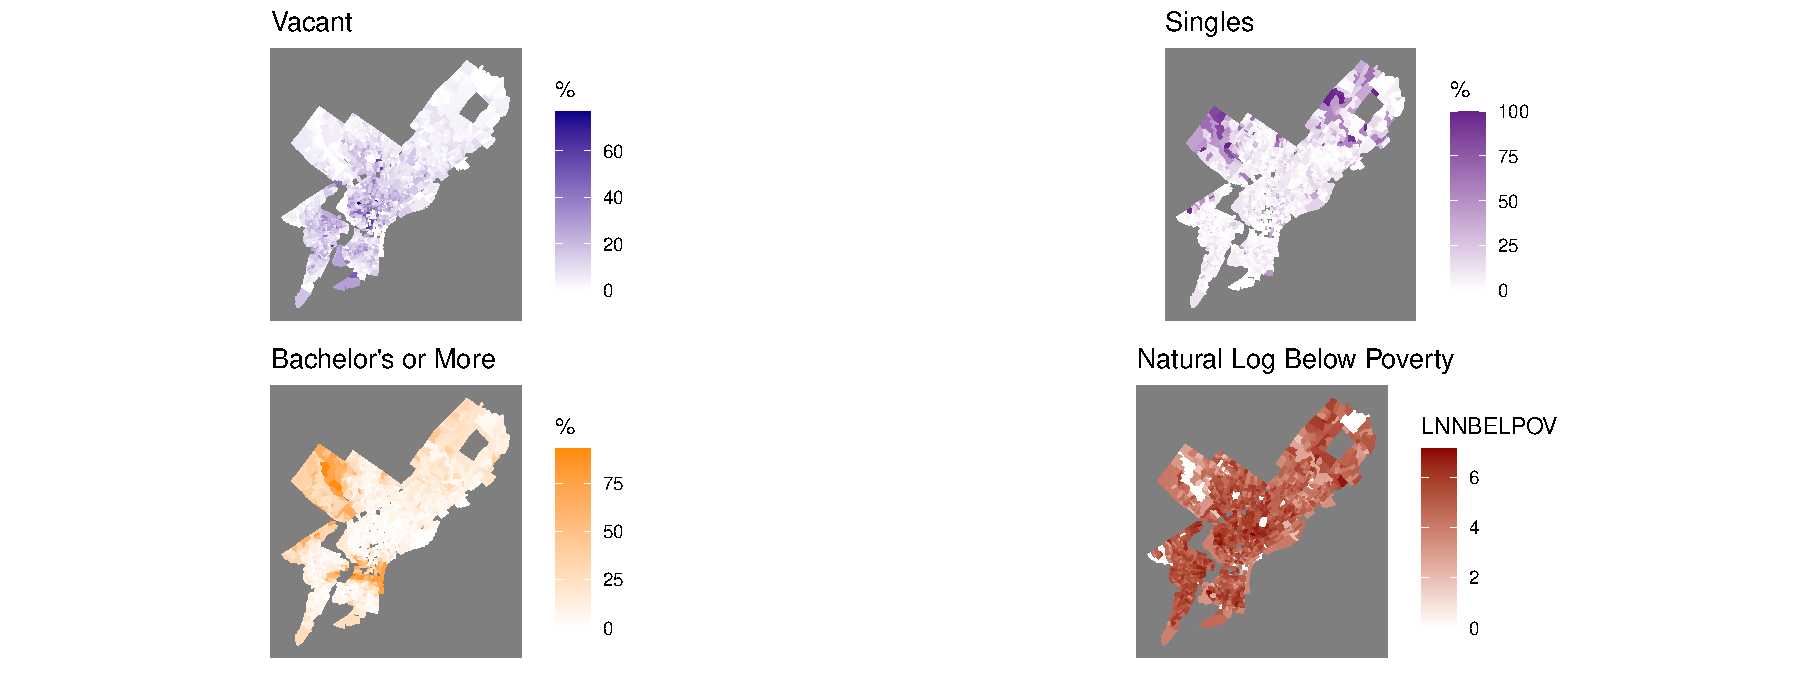
\includegraphics{HW1-Regression_files/figure-latex/variables maps-1.pdf}

\hypertarget{pearson-correlations}{%
\subsubsection{Pearson correlations}\label{pearson-correlations}}

The correlation matrix shows the Pearson correlation between each of our
dependent variables. For example, PCTBACHMOR is negatively correlated
with LNBELPOV100 and PCTVACANT is positively correlated with
LNBELPOV100.

Despite the correlations, we can conclude that there is not severe
multicollinearity. This is because the Pearson correlation values are
all between 0.8 and -0.8, which is considered an acceptable range when
considering multicollinearity.

The Pearson correlation value for the relationship between PCTBACHMOR
and PCTVACANT is -0.3, supporting our previous conclusion that there is
a negative correlation between the variables. However, the Pearson
correlation is within the acceptable range -0.8 to 0.8.

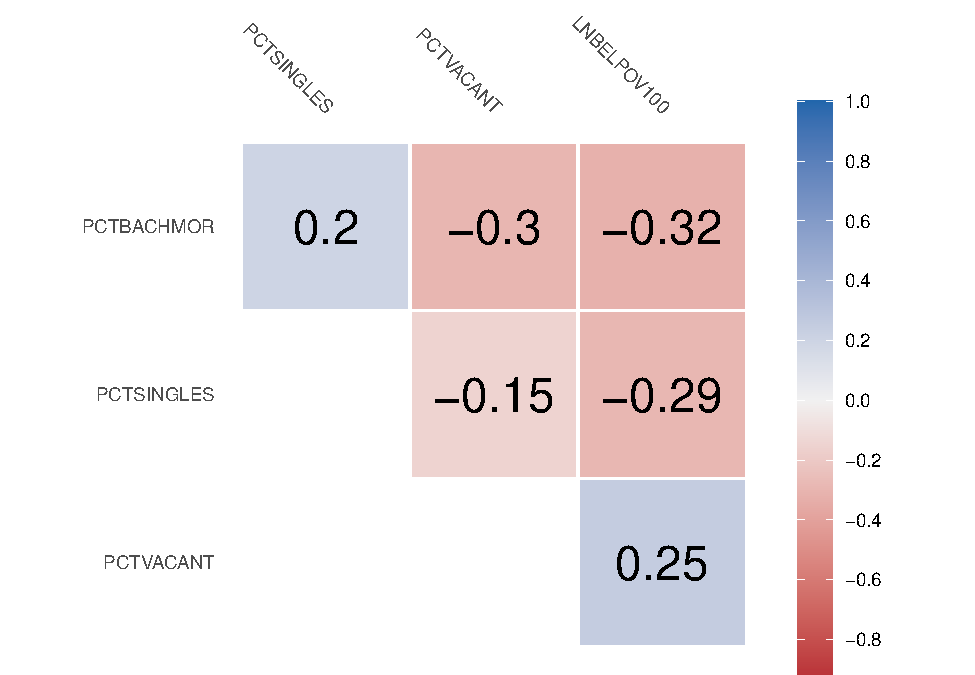
\includegraphics{HW1-Regression_files/figure-latex/pearson-1.pdf}

\hypertarget{regression-analysis}{%
\subsection{Regression Analysis}\label{regression-analysis}}

We first examine the f-ratio of our regression analysis. The f-ratio is
840.9, and the p-value associated with the f-ratio is less than 0.0001.
Thus, we can reject the null hypothesis that all β coefficients are
zero, and at least one of our independent variables is considered
statistically significant.

After reviewing the f-ratio, we consider the β coefficients, standard
errors, t statistics, and p-values for our four independent variables.
All four independent variables have a low enough p-value to consider
them statistically significant (\textless0.05) and we can reject the
null hypotheses that any of our β coefficients are equal to 0.

Based on our rejection of the null hypotheses, we can conclude the
following for block groups in our model:

\begin{itemize}
\tightlist
\item
  There is a statistically significant negative relationship between the
  natural log of the median home value and both of our independent
  variables for the proportion of homes which are vacant and the natural
  log of the number of households living in poverty.
\item
  There is a statistically significant positive relationship between the
  natural log of the median home value and both of our independent
  variables for the proportion of homes which are single family homes
  and the percent of individuals with a bachelor's degree.
\end{itemize}

When reviewing our Beta coefficient, we must consider the effects of the
natural log transformation on our dependent variable. For the predictors
proportion of homes which are standalone single family homes, proportion
of homes which are vacant, and percent of individuals with a bachelor
degree, only the dependent variable is natural log transformed. The Beta
coefficients are also less than 0.3. Thus, we can conclude that as our
independent variables increase by 1 unit, the expected change in median
home value is approximately \(100𝛽_1%
\):

\begin{itemize}
\tightlist
\item
  As the proportion of homes which are vacant goes up by 1\%, the median
  home value will decrease by approximately 1.916\%.
\item
  As the proportion of homes which are detached single family homes goes
  up by 1\% the median home value will increase by approximately
  0.298\%.
\item
  As the percentage of individuals who have a bachelor's degree goes up
  by 1\%, the median home value will increase by approximately 2.091\%.
\end{itemize}

For the population below the poverty line, both our independent variable
and our dependent variable are natural log-transformed. Thus, as the
population below the poverty line increases by 1, the median home value
will change by approximately \((1.01^𝛽_1 −1)∙100%
\), i.e: the median home value will decrease by approximately 0.07848\%.

The R-squared value is 0.6623, indicating that 66.23\% of the variance
in our dependent variable is explained by our four independent
variables. 33.77\% of the variance is not explained by our four
independent variables. Our adjusted R-squared value is 0.6615,
indicating that 66.15\% of the variance in our dependent variable is
explained by our four independent variables after adjusting the
r-squared to account for the model including more than one independent
variable.

\begin{verbatim}
## 
## Call:
## lm(formula = LNMEDHVAL ~ PCTVACANT + PCTSINGLES + PCTBACHMOR + 
##     LNBELPOV100, data = data)
## 
## Residuals:
##      Min       1Q   Median       3Q      Max 
## -2.25825 -0.20391  0.03822  0.21744  2.24347 
## 
## Coefficients:
##               Estimate Std. Error t value             Pr(>|t|)    
## (Intercept) 11.1137661  0.0465330 238.836 < 0.0000000000000002 ***
## PCTVACANT   -0.0191569  0.0009779 -19.590 < 0.0000000000000002 ***
## PCTSINGLES   0.0029769  0.0007032   4.234            0.0000242 ***
## PCTBACHMOR   0.0209098  0.0005432  38.494 < 0.0000000000000002 ***
## LNBELPOV100 -0.0789054  0.0084569  -9.330 < 0.0000000000000002 ***
## ---
## Signif. codes:  0 '***' 0.001 '**' 0.01 '*' 0.05 '.' 0.1 ' ' 1
## 
## Residual standard error: 0.3665 on 1715 degrees of freedom
## Multiple R-squared:  0.6623, Adjusted R-squared:  0.6615 
## F-statistic: 840.9 on 4 and 1715 DF,  p-value: < 0.00000000000000022
\end{verbatim}

The table below shows an analysis of the variance table for our linear
regression model. The Sum of Square Errors (SSE) for our model is
230.44. The Regression Sum of Squares (SSR) is equal to 451.745, and the
Total Sum of Squares (SST) is equal to 672.185. We can calculate the
\(R^2\) for our model by dividing the SSR by the SST, i.e: 451.745 /
682.089 which equals 0.6623.

\begin{verbatim}
## Analysis of Variance Table
## 
## Response: LNMEDHVAL
##               Df  Sum Sq Mean Sq  F value                Pr(>F)    
## PCTVACANT      1 180.392 180.392 1343.087 < 0.00000000000000022 ***
## PCTSINGLES     1  24.543  24.543  182.734 < 0.00000000000000022 ***
## PCTBACHMOR     1 235.118 235.118 1750.551 < 0.00000000000000022 ***
## LNBELPOV100    1  11.692  11.692   87.054 < 0.00000000000000022 ***
## Residuals   1715 230.344   0.134                                   
## ---
## Signif. codes:  0 '***' 0.001 '**' 0.01 '*' 0.05 '.' 0.1 ' ' 1
\end{verbatim}

\hypertarget{regression-assumptions-checks}{%
\subsection{Regression Assumptions
Checks}\label{regression-assumptions-checks}}

In this section, we will discuss testing model assumptions. We have
already examined the variable distributions in a prior section.

\hypertarget{scatter-plots---linear-relationships-between-variables}{%
\subsubsection{Scatter Plots - Linear Relationships Between
Variables}\label{scatter-plots---linear-relationships-between-variables}}

When running linear regressions, a core assumption is that there is a
linear relationship between the dependent variable and each of the
predictor variables. To check this assumption, we plot the dependent
variable with each of the predictor variables in a scatter plot.

In cases where this assumption is not met, log transformations are often
used. Based on the results of our variable distributions, we have
already conducted log transformations for the dependent variable for
median home value, now LNMEDHVAL, and for the predictor variable for
number of households below poverty, now LNNBELPOV100.

The following scatter plots show the relationship between the dependent
variable, LNMEDHVAL, and each of the predictor variables LNNBELPOV100,
PCTBACHMOR, PCTVACANT, and PCTSINGLES. There does not appear to be a
linear relationship between LNMEDHVAL and the predictor variables, even
with log transformations used. The variables all appear heavily skewed -
the relationship between LNNBELPOV and LNBELPOV100 appears to be
negatively skewed, and the individual relationship between the other
three predictors and LNMEDHVAL appears to be heavily positively skewed.

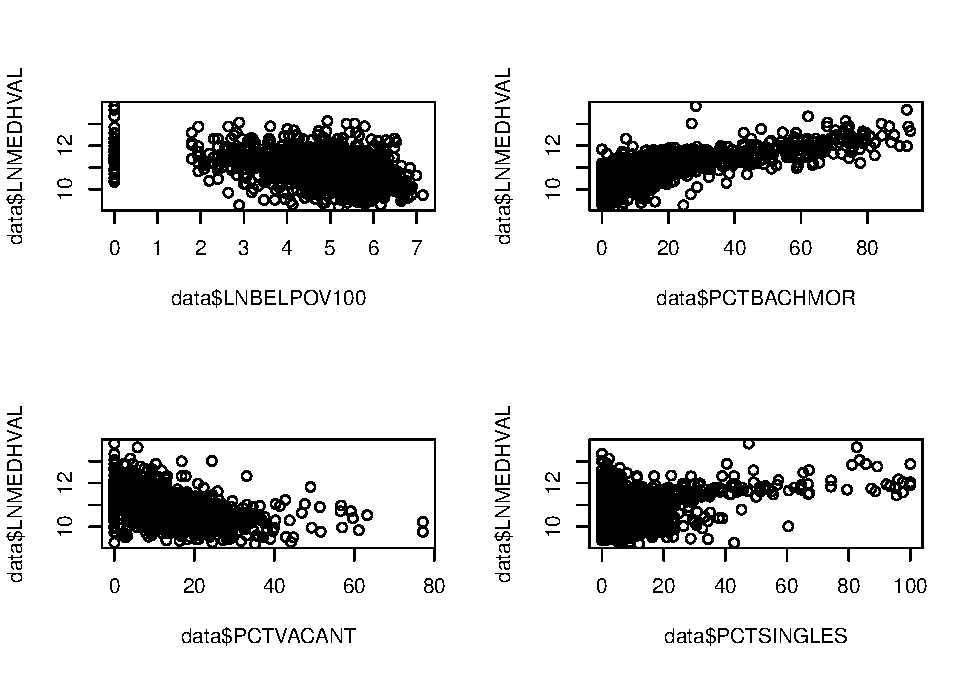
\includegraphics{HW1-Regression_files/figure-latex/scatter-1.pdf}

\hypertarget{histogram-of-the-standardized-residuals}{%
\subsubsection{Histogram of the standardized
residuals}\label{histogram-of-the-standardized-residuals}}

Another assumption when running linear regression is that regression
residuals are distributed normally. However, this assumption of
normality is not considered critical in a regression, especially for
data sets with a large number of observations.

In order to compare residuals for different observations, we standardize
the residuals through dividing a residual by its standard error.
Standardizing allows us to observe how many standard deviations a
residual is from our model's estimate

The following histogram of standardized residuals shows that residuals
appear normally distributed.

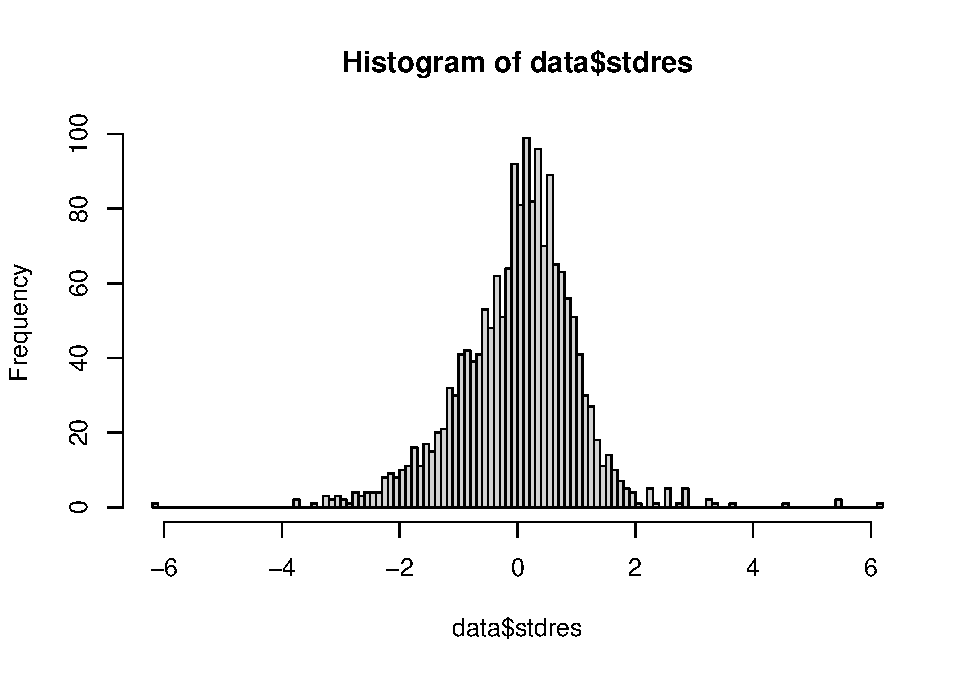
\includegraphics{HW1-Regression_files/figure-latex/resid plot-1.pdf}

\hypertarget{scatter-plot---standardized-residual-by-predicted-value}{%
\subsubsection{Scatter Plot - Standardized Residual by Predicted
Value}\label{scatter-plot---standardized-residual-by-predicted-value}}

An additional core assumption of linear regression is that there is
constant variance in residuals compared to the predicted values of the
model - this relationship is referred to as homoscedastic. If
non-constant variance is observed, the relationship is heteroscedastic.

Given that there are multiple predictors, we can plot the standardized
residuals of the model by our predicted values of LNMEDHVAL. The scatter
plot of standardized residuals appears to show a slight heteroscedastic
relationship, based on a small ``bow-tie'' shape present around the
predicted value of 11.5.

Outliers also appear to be present based on our scatter plot - there are
several positive standardized residuals above 4 standard deviations
above 0 and at least one standardized residual beyond -6 standard
deviation below 0.

The standardized residuals also appear to be heavily clustered around
between the predicted values of about 10.5 to 11.5.

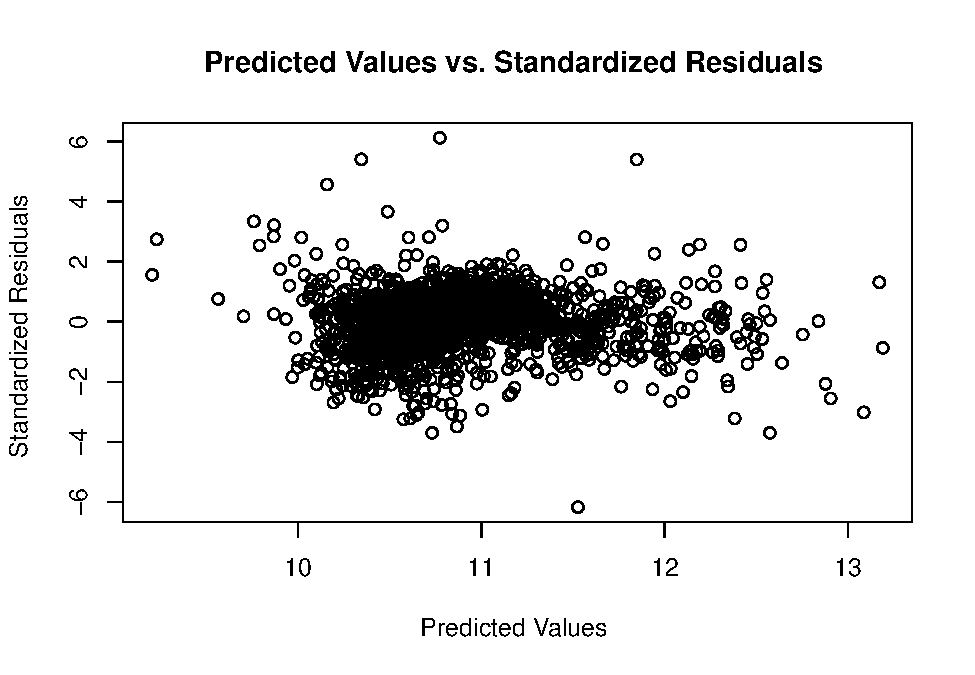
\includegraphics{HW1-Regression_files/figure-latex/plot_stand_resid-1.pdf}

\hypertarget{spatial-autocorrelation-of-variables}{%
\subsubsection{Spatial Autocorrelation of
Variables}\label{spatial-autocorrelation-of-variables}}

Based on the maps of the dependent variable LNMEDHVAL and the predictor
variables, we can estimate whether observations of each variable appear
to show spatial autocorrelation - defined as observing the degree to
which similar values cluster near each other. Our variables may appear
to spatial autocorrelation

A critical assumption when building a regression model is that each
observation of a variable is independent from other observations of that
variable which we examine in our variables as spatial dependence,
otherwise known as spatial autocorrelation. Based on the maps of the
dependent variable LNMEDHVAL and the predictor variables, we can
estimate whether observations of each variable appear to show spatial
autocorrelation, which would appear as block groups clustering with
similar values:

\begin{itemize}
\tightlist
\item
  The log of median home values appears to show spatial autocorrelation.
  High values appear to cluster in the downtown area and northwest
  Philadelphia, while low values appear to cluster around North
  Philadelphia and southwest Philadelphia, among other areas.
\item
  Vacancy percentages appear to cluster in similar areas as the low
  value clusters of the log of median home values - North Philadelphia
  and southwest Philadelphia.
\item
  Singles percentages appear to cluster in the northwest and northeast
  regions of the city.
\item
  Bachelor's degree or more percentages appear to cluster in similar
  areas to the high values of the log of median home values - the
  downtown area and northwest Philadelphia.
\item
  The log of the number of households in poverty does not appear to show
  spatial autocorrelation.
\end{itemize}

Based on these maps, each of the variables in our regression model
appear to show spatial autocorrelation.

\hypertarget{choropleth-map-of-the-standardized-regression-residuals}{%
\subsubsection{Choropleth map of the standardized regression
residuals}\label{choropleth-map-of-the-standardized-regression-residuals}}

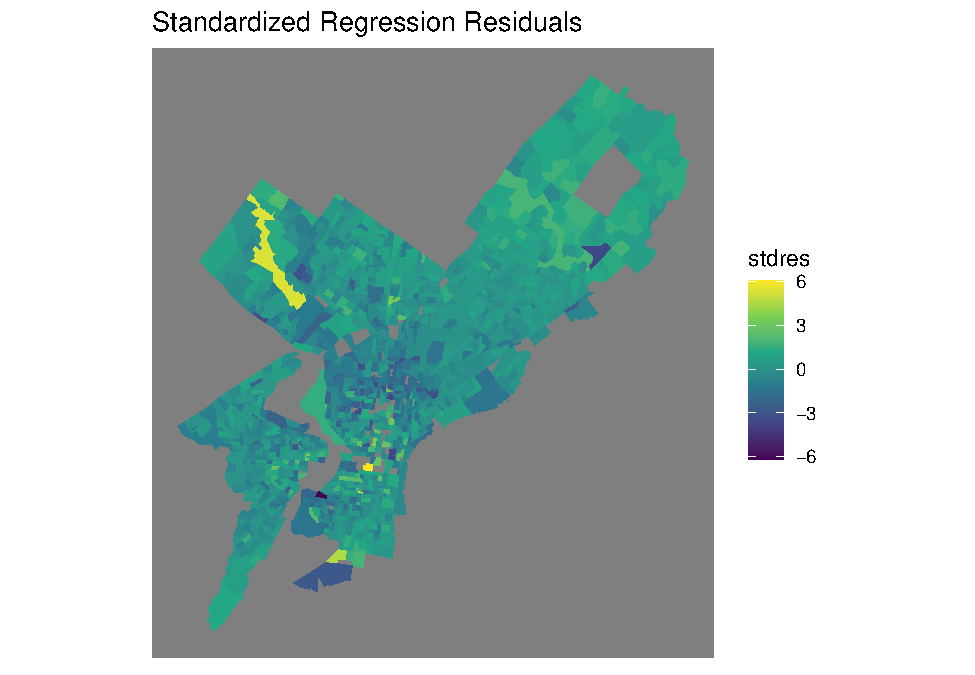
\includegraphics{HW1-Regression_files/figure-latex/resid map-1.pdf}

\hypertarget{additional-models}{%
\subsection{Additional Models}\label{additional-models}}

\hypertarget{stepwise-regression-1}{%
\subsubsection{Stepwise Regression}\label{stepwise-regression-1}}

Inputting the variables of our model into a stepwise regression test
results in a final model that retains all four of the original predictor
variables. Therefore, all four predictors had sufficiently low p-values
and removing predictors did not lower the value of the AIC.

\begin{verbatim}
## Start:  AIC=-3448.07
## LNMEDHVAL ~ PCTVACANT + PCTSINGLES + PCTBACHMOR + LNBELPOV100
## 
##               Df Sum of Sq    RSS     AIC
## <none>                     230.34 -3448.1
## - PCTSINGLES   1     2.407 232.75 -3432.2
## - LNBELPOV100  1    11.692 242.04 -3364.9
## - PCTVACANT    1    51.546 281.89 -3102.7
## - PCTBACHMOR   1   199.020 429.36 -2379.0
\end{verbatim}

\begin{verbatim}
## Stepwise Model Path 
## Analysis of Deviance Table
## 
## Initial Model:
## LNMEDHVAL ~ PCTVACANT + PCTSINGLES + PCTBACHMOR + LNBELPOV100
## 
## Final Model:
## LNMEDHVAL ~ PCTVACANT + PCTSINGLES + PCTBACHMOR + LNBELPOV100
## 
## 
##   Step Df Deviance Resid. Df Resid. Dev       AIC
## 1                       1715   230.3435 -3448.073
\end{verbatim}

\hypertarget{cross-validation}{%
\subsubsection{Cross-Validation}\label{cross-validation}}

The following table provides the results of k-fold cross validation,
when the number of folds (k) is set to 5. The root mean square error of
the original model is represented by rmse1, which we compare to a second
regression model's root mean square error, rmse2. This second model only
includes the percent of vacancy and median household income as
predictors for median home value. Given that rmse1 is lower than rmse2,
our original model is considered more generalizable when using different
folds of the data and is thus a better fit for the model.

\hypertarget{discussion-and-limitations}{%
\section{Discussion and Limitations}\label{discussion-and-limitations}}

Based on our model we can conclude that there is a statistically
significant relationship between our dependent variable, the natural log
of the median home value and our four dependent variables. We can
conclude that areas of Philadelphia where a larger number of residents
live in poverty, residents do not have higher education degrees, and a
large number of vacant homes are present are likely to also have a low
median home value.

This conclusion was not surprising, as poorer households are likely to
only be able to afford homes in areas with lower median home values.
Additionally, redlining during the mid 1900s in Philadelphia identified
undesirable neighborhoods. Redlining has a lasting impact on the
Philadelphia housing landscape. Neighborhoods which were identified as
undesirable continue to have higher vacancy rates and house low income
households.

Our model does a good job explaining the variation in median home value
across the city of Philadelphia. The results of the F-test indicate that
all our dependent variables are statistically significant predictors of
median home value. Our R\^{}2 value of 0.6623 indicates there is a
strong linear correlation between our independent variables and the
natural log of the median home sales value. We consider a R\^{}2 value
above 0.5 to be indicative of a strong correlation, the 0.5 threshold
core a strong correlation is acceptable in the social sciences domain.

Our stepwise regression model included all four of the original
predictor variables. Therefore, all four variables are considered
statistically significant predictors of our dependent variable, the
natural log of median home values, and our model performs best with all
four predictors included as opposed to some subset of the independent
variables.

Several core assumptions of OLS regressions are violated by our model.
Our predictor variables do not all appear to have linear relationships
with our dependent variable - namely LNNBELPOV100, PCTVACANT, and
PCTSINGLES. Natural log transformations were used for the dependent
variable and the number of households below poverty, but the non-linear
relationships still appear. The variance of the residuals also appears
to be heteroscedastic, which likely means that our model systematically
underperforms in certain areas of the city based on characteristics not
accounted for in our model. The predictor variables also appear to show
potential spatial autocorrelation, which our model does not account for
and could explain the heteroscedasticity of our residuals.

The predictor variable NBELPOV100 is the only independent variable that
is provided as a raw number as opposed to a percentage that normalizes
the values to compare across block groups. Block groups with smaller
counts of population would experience an outsized impact in the
regression model by increasing the count by one household, whereas block
groups with larger populations would not experience the same level of
impact. Normalizing to percentages allows us to compare 1 percent
increases, representing proportional impacts to different block groups.

Our cross-validation results show that the root mean square error for
the four predictor model was lower than that of the two predictor model,
identifying the former model as better and more generalizable for new
data.

Ridge Regression is a method that offers solutions to issues that can
arise in OLS Regression such as: allowing for a large number of
predictors relative to the number of observations, allows for
multicollinearity, and deals with overfitting by shrinking the
coefficients of variables towards 0 (which can significantly reduce
their variance and the RMSE in the validation set). Ridge regression
functions by minimizing the SSE subject to a found (i.e., constraint) on
the on the quantity called L2 norm (the square root of the sum of the
squared β coefficients) where in OLS we minimize the SSE.

Lasso Regression (least absolute shrinkage \& selection operator), is
like ridge regression except that it will set the values of some
coefficients to exactly 0 for different values of λ, minimizing SSE
subject to a bound on the quantity called L1 norm (the sum of absolute
values of the β coefficients). Both ridge and lasso regression would not
be appropriate here because they drop the assumption of no
multicollinearity. When this assumption is violated, we can get
incorrect estimates of \(β_i\) as well as incorrect estimates of
p-values of significance.

\end{document}
